
\documentclass[12pt]{article}
\usepackage[english,russian]{babel}
\usepackage{graphicx}
\usepackage{xcolor}


\begin{document}


\Large Отчет по лабораторной работе №22 по курсу "Фундаментальная информатика"
\normalsize

{\bfseries Студент группы:} M8O-108Б-22 Сибирцев Роман Денисович

{\bfseries Контакты e-mail:} sibirtsevr1@gmail.com

{\bfseries Работа выполнена:} «12» апреля 2023 г. 

{\bfseries Преподаватель:} асп. каф. 806 Сахарин Никита Александрович

{\bfseries Входной контроль знаний с оценкой:}

{\bfseries Отчет сдан} «8» апреля 2023 г., {\bfseries итоговая оценка:}

{\bfseries Подпись преподавателя:} \underline{\hspace{3cm}}


{\Large 1. Тема}

{\itshape Издательская система \TeX}

{\Large 2. Цель работы}

{\itshape Изучить оформление документов в системе \TeX}

{\Large 3. Задание}

Оформить отчет в \TeX

{\Large 4. Оборудование}


{\bfseries Прицессор:} AMD Ryzen 5 3600 (12) @ 3.600GHz

{\bfseries ОП:} 15944MiB

{\bfseries HDD:} 1TB

{\Large 5. Программное обеспечение}


{\bfseries Операционная система семейства} {\itshape UNIX}

{\bfseries наименование} {\itshape Arch Linux}, {\bfseries версия} {\itshape 6.2.2-arch1-1} 

{\bfseries Интерпритатор команд} {bash}, {\bfseries версия} {5.1.16} 

{\bfseries Редактор текстов} {\itshape nano}

{\Large 6. Идея, метод, алгоритм}

Прочитать документацию \TeX

Написать отчет с помощбю системы форматирования \TeX


{\Large 7. Сценарий выполнения работы}

\begin{equation}
\mathcal{L}(\theta) = 0.1 \|\theta\|^2 + \frac{1}{N}\sum\limits_{i=1}^N \max(0, 1 - y_i f(x_i, \theta))
\end{equation}

\begin{equation}
A_{n \times n} = \left(
\begin{array}{cccc}
a_{11} & a_{12} & \ldots & a_{1n}\\
a_{21} & a_{22} & \ldots & a_{2n}\\
\vdots & \vdots & \ddots & \vdots\\
a_{n1} & a_{n2} & \ldots & a_{nn}
\end{array}
\right)
\end{equation}

% GNUPLOT: LaTeX picture with Postscript
\begingroup
  \makeatletter
  \providecommand\color[2][]{%
    \GenericError{(gnuplot) \space\space\space\@spaces}{%
      Package color not loaded in conjunction with
      terminal option `colourtext'%
    }{See the gnuplot documentation for explanation.%
    }{Either use 'blacktext' in gnuplot or load the package
      color.sty in LaTeX.}%
    \renewcommand\color[2][]{}%
  }%
  \providecommand\includegraphics[2][]{%
    \GenericError{(gnuplot) \space\space\space\@spaces}{%
      Package graphicx or graphics not loaded%
    }{See the gnuplot documentation for explanation.%
    }{The gnuplot epslatex terminal needs graphicx.sty or graphics.sty.}%
    \renewcommand\includegraphics[2][]{}%
  }%
  \providecommand\rotatebox[2]{#2}%
  \@ifundefined{ifGPcolor}{%
    \newif\ifGPcolor
    \GPcolortrue
  }{}%
  \@ifundefined{ifGPblacktext}{%
    \newif\ifGPblacktext
    \GPblacktextfalse
  }{}%
  % define a \g@addto@macro without @ in the name:
  \let\gplgaddtomacro\g@addto@macro
  % define empty templates for all commands taking text:
  \gdef\gplbacktext{}%
  \gdef\gplfronttext{}%
  \makeatother
  \ifGPblacktext
    % no textcolor at all
    \def\colorrgb#1{}%
    \def\colorgray#1{}%
  \else
    % gray or color?
    \ifGPcolor
      \def\colorrgb#1{\color[rgb]{#1}}%
      \def\colorgray#1{\color[gray]{#1}}%
      \expandafter\def\csname LTw\endcsname{\color{white}}%
      \expandafter\def\csname LTb\endcsname{\color{black}}%
      \expandafter\def\csname LTa\endcsname{\color{black}}%
      \expandafter\def\csname LT0\endcsname{\color[rgb]{1,0,0}}%
      \expandafter\def\csname LT1\endcsname{\color[rgb]{0,1,0}}%
      \expandafter\def\csname LT2\endcsname{\color[rgb]{0,0,1}}%
      \expandafter\def\csname LT3\endcsname{\color[rgb]{1,0,1}}%
      \expandafter\def\csname LT4\endcsname{\color[rgb]{0,1,1}}%
      \expandafter\def\csname LT5\endcsname{\color[rgb]{1,1,0}}%
      \expandafter\def\csname LT6\endcsname{\color[rgb]{0,0,0}}%
      \expandafter\def\csname LT7\endcsname{\color[rgb]{1,0.3,0}}%
      \expandafter\def\csname LT8\endcsname{\color[rgb]{0.5,0.5,0.5}}%
    \else
      % gray
      \def\colorrgb#1{\color{black}}%
      \def\colorgray#1{\color[gray]{#1}}%
      \expandafter\def\csname LTw\endcsname{\color{white}}%
      \expandafter\def\csname LTb\endcsname{\color{black}}%
      \expandafter\def\csname LTa\endcsname{\color{black}}%
      \expandafter\def\csname LT0\endcsname{\color{black}}%
      \expandafter\def\csname LT1\endcsname{\color{black}}%
      \expandafter\def\csname LT2\endcsname{\color{black}}%
      \expandafter\def\csname LT3\endcsname{\color{black}}%
      \expandafter\def\csname LT4\endcsname{\color{black}}%
      \expandafter\def\csname LT5\endcsname{\color{black}}%
      \expandafter\def\csname LT6\endcsname{\color{black}}%
      \expandafter\def\csname LT7\endcsname{\color{black}}%
      \expandafter\def\csname LT8\endcsname{\color{black}}%
    \fi
  \fi
    \setlength{\unitlength}{0.0500bp}%
    \ifx\gptboxheight\undefined%
      \newlength{\gptboxheight}%
      \newlength{\gptboxwidth}%
      \newsavebox{\gptboxtext}%
    \fi%
    \setlength{\fboxrule}{0.5pt}%
    \setlength{\fboxsep}{1pt}%
    \definecolor{tbcol}{rgb}{1,1,1}%
\begin{picture}(7200.00,5040.00)%
    \gplgaddtomacro\gplbacktext{%
      \csname LTb\endcsname%%
      \put(963,1308){\makebox(0,0){\strut{}$-10$}}%
      \put(1773,1160){\makebox(0,0){\strut{}$-5$}}%
      \put(2583,1011){\makebox(0,0){\strut{}$0$}}%
      \put(3392,863){\makebox(0,0){\strut{}$5$}}%
      \put(4201,714){\makebox(0,0){\strut{}$10$}}%
      \put(4427,746){\makebox(0,0)[l]{\strut{}$-10$}}%
      \put(4895,1004){\makebox(0,0)[l]{\strut{}$-5$}}%
      \put(5362,1261){\makebox(0,0)[l]{\strut{}$0$}}%
      \put(5830,1518){\makebox(0,0)[l]{\strut{}$5$}}%
      \put(6297,1775){\makebox(0,0)[l]{\strut{}$10$}}%
      \put(920,1384){\makebox(0,0)[r]{\strut{}$0$}}%
      \put(920,1590){\makebox(0,0)[r]{\strut{}$1000$}}%
      \put(920,1796){\makebox(0,0)[r]{\strut{}$2000$}}%
      \put(920,2002){\makebox(0,0)[r]{\strut{}$3000$}}%
      \put(920,2207){\makebox(0,0)[r]{\strut{}$4000$}}%
      \put(920,2413){\makebox(0,0)[r]{\strut{}$5000$}}%
      \put(920,2619){\makebox(0,0)[r]{\strut{}$6000$}}%
      \put(920,2824){\makebox(0,0)[r]{\strut{}$7000$}}%
      \put(920,3029){\makebox(0,0)[r]{\strut{}$8000$}}%
      \put(920,3235){\makebox(0,0)[r]{\strut{}$9000$}}%
      \put(920,3441){\makebox(0,0)[r]{\strut{}$10000$}}%
    }%
    \gplgaddtomacro\gplfronttext{%
      \csname LTb\endcsname%%
      \put(5955,4536){\makebox(0,0)[r]{\strut{}$(x**2)*(y**2)$}}%
    }%
    \gplbacktext
    \put(0,0){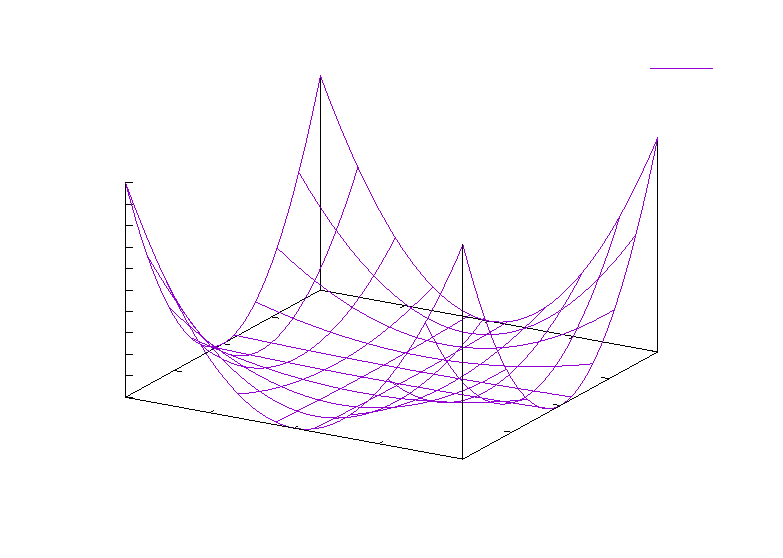
\includegraphics[width={360.00bp},height={252.00bp}]{graph}}%
    \gplfronttext
  \end{picture}%
\endgroup



{\Large 8. Распечатка протокола}


\begin{verbatim}
[roman@archlinux lab_22]$ ls
graph.eps graph-eps-converted-to.pdf graph.tex report.tex
[roman@archlinux lab_22]$ latex report.tex 
This is pdfTeX, Version 3.141592653-2.6-1.40.25 (TeX Live 2023/Arch Linux) 
(preloaded format=latex)
 restricted \write18 enabled.
entering extended mode
(./report.tex
LaTeX2e <2022-11-01> patch level 1
L3 programming layer <2023-02-22>
(/usr/share/texmf-dist/tex/latex/base/article.cls
Document Class: article 2022/07/02 v1.4n Standard LaTeX document class
(/usr/share/texmf-dist/tex/latex/base/size12.clo))
(/usr/share/texmf-dist/tex/generic/babel/babel.sty
(/usr/share/texmf-dist/tex/generic/babel/txtbabel.def)
(/usr/share/texmf-dist/tex/generic/babel-english/english.ldf)
(/usr/share/texmf-dist/tex/generic/babel-russian/russianb.ldf

Package babel Warning: No Cyrillic font encoding has been loaded so far.
(babel)                A font encoding should be declared before babel.
(babel)                Default `T2A' encoding will be loaded  on input line 78.


(/usr/share/texmf-dist/tex/latex/cyrillic/t2aenc.def
(/usr/share/texmf-dist/tex/latex/base/t2aenc.dfu))))
(/usr/share/texmf-dist/tex/generic/babel/locale/ru/babel-russian.tex)
(/usr/share/texmf-dist/tex/generic/babel/locale/en/babel-english.tex)
(/usr/share/texmf-dist/tex/latex/graphics/graphicx.sty
(/usr/share/texmf-dist/tex/latex/graphics/keyval.sty)
(/usr/share/texmf-dist/tex/latex/graphics/graphics.sty
(/usr/share/texmf-dist/tex/latex/graphics/trig.sty)
(/usr/share/texmf-dist/tex/latex/graphics-cfg/graphics.cfg)
(/usr/share/texmf-dist/tex/latex/graphics-def/dvips.def)))
(/usr/share/texmf-dist/tex/latex/xcolor/xcolor.sty
(/usr/share/texmf-dist/tex/latex/graphics-cfg/color.cfg)
(/usr/share/texmf-dist/tex/latex/graphics/mathcolor.ltx))
(/usr/share/texmf-dist/tex/latex/l3backend/l3backend-dvips.def)
No file report.aux.
(/usr/share/texmf-dist/tex/latex/cyrillic/t2acmr.fd)
Overfull \hbox (0.17178pt too wide) in paragraph at lines 10--12
(./graph.tex <graph.eps>) [1] [2] (./report.aux) )
(see the transcript file for additional information)
Output written on report.dvi (2 pages, 4328 bytes).
Transcript written on report.log.
[roman@archlinux lab_22]$ ls
graph.eps graph-eps-converted-to.pdf graph.tex report.aux report.dvi report.log 
report.tex
[roman@archlinux lab_22]$ divpdf report.dvi 
bash: divpdf: command not found
[roman@archlinux lab_22]$ dvipdf report.dvi 
[roman@archlinux lab_22]$ ls
graph.eps graph-eps-converted-to.pdf graph.tex report.aux report.dvi report.log 
report.pdf  report.tex
\end{verbatim}



\newpage
{\Large 9. Дневник отдадки}

\begin{tabular}{|c|c|c|c|c|c|c|}
\hline
№ & Лаб. & Дата & Время & Событие & Действие по & Привмечание\\ 
&или & & & & справлению & \\ 
&дом. & & & & & \\
\hline
1 & дом. & 12.04.23 & 15:00 & Выполнение  & - & -\\
& & & & лабораторной & & \\
& & & & работы & & \\
\hline
\end{tabular}


{\Large 10. Замечания автора по существу работы}


{\Large 11. Выводы}

Были получены навыки оформления документов в системе \TeX.

{\bfseries Подпись студента:} \underline{\hspace{3cm}}

\end{document}